\section{Implementation}\label{sec:implementation}


\subsection{General Strategy}

Signature verification could be done by training a Convolutional Neural Network (CNN) to output whether or not the input image is of the chosen person.
However, this requires a new network to be trained for each person that the system needs to perform verification for.
Not only is it computationally very expensive to train such a system to perform verification for many people, but also requires many signatures by the person for training.

Instead, a high-level representation of the image can be found that includes only the information needed to distinguish people.
This is effectively dimensionality reduction that preserves only the information that is important for identifying people.
The high-level representation is a vector in what is referred to as a latent space.
(So, the dimensionality reduction should extract the structure of the person's face while discarding information about the background and the lighting conditions.)

This idea has a long history for face verification\cite{LeCun}, and has been used for signature verification much more recently in SigNet\cite{sig_net}.

We will start with the SigNet architecture, modify it in several ways, and then test its accuracy on skilled forges (handwritten forges by humans) and the same forges after modifying them using FGSM.


\subsection{Procedure}

For implementing the data preparation and SigNet architecture, 3 resources were used.
An existing PyTorch implementation of SigNet, \cite{GitHub_signet_pytorch}, was used as a starting place.
The SigNet paper, \cite{sig_net}, was used to check that the implementation was correct.
For a few details, the paper was ambiguous, so a Keras implementation, \cite{GitHub_sounakdey} which appears to be written by one of the paper's authors was used for clarification.

The existing PyTorch implementation was first restructured into a Jupyter Notebook so that it could be easily run on Google Colaboratory.

The SigNet papers describes experiments on several datasets, but only achieves 100\% accuracy on the CEDAR dataset.
For simplicity and reduced training time, only the CEDAR is used in this paper.
% todo ref CEDAR

The dataset was partitioned and prepared as described in the SigNet paper (which is very similar to \cite{LeCun}).

The existing training process did not implement data normalization, so this was implemented as per the paper.
The mean and standard deviation of the images in the training dataset was computed (after splitting the images in the CEDAR dataset into training and validation images and pairing images).
All of the images in the dataset were then resized, transformed (inverted), and normalized according the paper's description and then saved back into png files for efficient loading of the data on subsequent runs.
The png format was used rather than simply saving the tensors because png compression may perform better than the PyTorch (pt file) compression since png files are specific to images.

In an attempt to speed up the training process, all images are loaded in memory before training begins.
Rather than reading image data from disk, the dataloader simply indexes an array.
This is effective because there are many more training points (image pairs) than images, and it is feasible because the total uncompressed data in the images after they are resized is approximately 82 MB (2400 images of size 155 by 220 with pixels in range 0 to 255).

\subsubsection{Deviations from SigNet}
An error was found in the SigNet PyTorch implementation, fixed, and merged back into the codebase (\url{https://github.com/VinhLoiIT/signet-pytorch/pull/5}).

One discrepancy between SigNet and our implementation is the initialization of model weights.
The SigNet paper says that weights are initialized ``according to the work
of Glorot and Bengio \cite{glorot_bengio}, and the biases equal to 0''\cite{sig_net}.
Instead of porting the Keras code to PyTorch, the default PyTorch initialization is used.
The purpose of the weight initialization is to reduce convergence time.
Since the models converged quickly (the larger models perform better after only 5 epochs), this should invalidate results of experiments.
% this was largely to avoid re-running training, which took a long time
% dang, that paper says "we propose a new initialization scheme that brings substantially faster convergence"
% The models converged quickly, so this seems to be okay.

% All of the hyper-parameters are chosen to be the same as SigNet.
% except batch size, which is set to 1...

We speculate that the the latent vector size is an interesting factor for an ablation study.
To understand its importance, the size of SigNet's output was adjusted by modifying only the last layer.
The resulting networks have a 64, 128 (unchanged), and 256 dimensional outputs and are later referred to as SigNet64, SigNet128, and SigNet256, respectively.

\subsubsection{Training}
Training was done on Google Colab (using "Colab Pro" with a "High RAM" and GPU runtime).
Unfortunately, weights from a trained SigNet model could not be found anywhere.
The training speed varied drastically, from approximately 32 minutes to 22 hours per epoch.

% batch size was set to 1 to avoid OOMs.
% I think this does impact the training process because of some normalization process during training...

% Several things slowed down training considerably.
% Having GPU RAM maxed out (I think).
% Initially, (with GPU RAM maxed out and not on a "High RAM" runtime) training an epoch took over 24 hours.
% At its best, training was able to do ~15 epochs in ~8 hours, which is 32 mins per epoch.


% \subsubsection{Loss}
The contrastive loss function is used exactly as in SigNet\cite{GitHub_sounakdey}.
% It was decided not to try using a triplet loss function for SigNet because it would be substantial work (mainly partitioning the data and dynamically selecting image triplets intelligently) and it seems that triplet loss is mainly useful for modelling more complex data when large compute resources are available.


\subsection{Experiments}

Experiments were conducted with the intent to validate the model as if it were used in a signature verification system, to understand how effective white-box attacks are, and to understand how latent vector size impacts the accuracy and robustness of the system.

\subsubsection{Threshold Strategy}\label{sec:threshold}
% This code was checked against the Keras implementation.

The code in the Keras implementation computes accuracy as the SigNet paper describes.
As mentioned in section \ref{sec:sig_net}, a threshold is selected by examining the validation set (and choosing the optimal threshold).
This approach is useful for understanding the potential of the SigNet architecture.
However, since the threshold is technically part of the classification system, information is leaked from the validation set.
As such, this threshold strategy is later referred to as being ``leaky''.
Therefore, the resulting accuracy does not technically demonstrate the accuracy that SigNet would have in the real world.

In this paper, the median distance for a genuine pair and for an impostor pair is computed on a sample of the training set.
The midpoint between the 2 medians is then used as the threshold distance.
The rationale for this over computing the optimal threshold for a sample of the training data is that it would hopefully generalize over the data better.

In figure \ref{fig:hist_distance} we can see that the data is very nicely separated (for SigNet128 trained for 20 epochs).
The ``median'' threshold distance is 0.0335 and the ``leaky'' threshold distance is 0.0402.
The ``leaky'' threshold is significantly different, but results in the system achieving only a slightly higher accuracy (99.67\% compared to 99.49\%) because the data is very well separated.
\begin{figure}[h]
    \begin{center}
        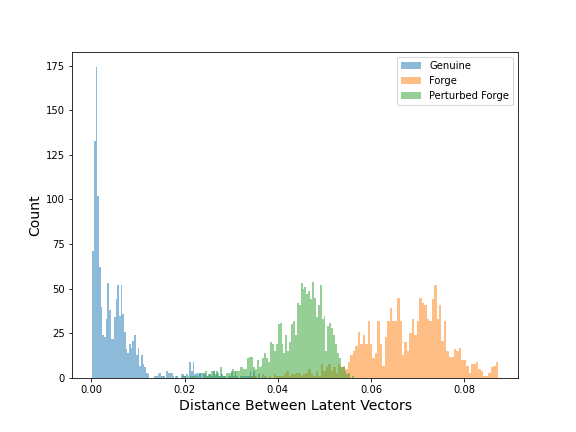
\includegraphics[width=0.8\linewidth]{distance_histogram_signet_128.png}
    \end{center}
    \caption{Histogram of Distances of Validation Set for SigNet128}
    \label{fig:hist_distances}
\end{figure}


% I should compute the divide as $p_same / (p_same + p_different)$ where each p is computed as the Gaussian distribution of the distances on the training data...

% !!! I don't think that SigNet implements the decision (genuine vs. forge) correctly !!!
% It treats all dimensions with equal weight, whereas LeCun computes the mean and cov mat of several genuine images and then computes p based on a Gaussian assumption.
% Yeah, SigNet just finds a threshold distance and uses that... (which naively weights all dimensions equally)

% compute mean and std\_dev of the distance between a matching and non-matching pair on a bunch of training points.

% I think that what I should implement (also) is compute the mean and covariance (matrices) of the genuine and forge data latent vectors over a bunch of training pairs. (To compute variance, I might need to store the latent vectors in CPU RAM and free the GPU RAM to avoid GPU OOM.)
% I can also compute the confusion matrix using the simple threshold distance and my thing and discuss the performance differences.

% Maybe I should also try what LeCun did with computing normal distribution for an individual and then using inverse FGSM (aka gradient descent on the input... could I use Pytorch optimizer and stuff for choosing a step value??? no!, don't bother)

% If I transfer the latent vectors to the CPU (and don't include the gradients!), then I can easily store the latent vectors for all of the training images!
% (should be 128 floats for each, but FaceNet paper says we can compress to 128 bytes ``without loss of accuracy'' ... but they don't say how exactly...)
% Then, I could compute the covariances of the clusters and also do some analytics on understanding the clusters.
% Yeah, memoizing the latent vectors when doing validation (and finding a threshold(s)) is a really good idea!

% Assume that both genuine pair distance vectors and impostor pair distance vectors are Gaussian, and then compare probabilities (computed using Bayes Theorem and Gaussian distributions).
% The comparison can simplified significantly like so:...

\subsubsection{FGSM Attack}\label{sec:my_fgsm}
A variation of the FGSM attack (described in section \ref{sec:fgsm}) is used to attack each SigNet model.
Latent vectors for a genuine and forge signature are computed using the model.
The gradient of the loss with respect to the forge image is computed, as in FGSM.
The loss function is computed as if the images are genuine, so the loss is the distance between the latent vectors (where dimensions that differ by less than 1 pixel step are ignored).
The gradient is scaled by some constant $\epsilon$, producing a perturbation.
The perturbation is then subtracted from the forge image to produce a perturbed (improved) forge.
Assuming the model behaves somewhat linearly, the perturbed forge should result in a small loss, so its latent vector will be close to the genuine's latent vector, hopefully fooling the signature verification system.

In the original paper on FGSM, 0.007 is used as the $\epsilon$ value because it corresponds to a perturbation that is a rounding error when averaged over the image.
More precisely, it is ``the magnitude of the smallest bit of an 8 bit image encoding after GoogLeNet's conversion to real numbers''\cite{goodfellow}.
For this paper, 0.004 (roughly 1/256) was used because each pixel takes a grayscale value from 0 to 255.
This $\epsilon$ value was used for all models in an attempt to have an apples-to-apples comparison.

Figure \ref{fig:dist_vs_perts} shows how the distance between latent vectors decreases with successive perturbations, re-computing the gradient each time.
It is evident that after approximately 4 perturbations the forge will not be distinguishable (using a simple distance metric) from the cluster of genuine signatures shown in figure \ref{fig:hist_distances}.
% what about a gaussian threshold strategy?
\begin{figure}[h]
    \begin{center}
        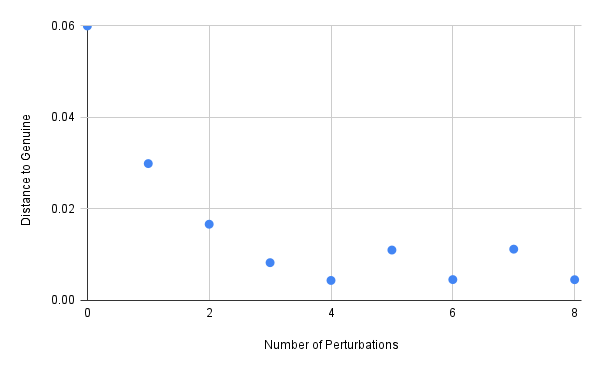
\includegraphics[width=0.8\linewidth]{dist_pert_plot.png}
    \end{center}
    \caption{Successive Perturbations on a Forgery}
    \label{fig:dist_vs_perts}
\end{figure}

Figure \ref{fig:genuine} shows the genuine signature used for this experiment and figure \ref{fig:forge} shows the forge.
There is a small, but noticeable difference between the forge and the perturbed forge (shown in figure \ref{fig:improved_forge}), but all successive forges are identical to the once perturbed forge to the human eye.
\begin{figure}[h]
    \begin{center}
        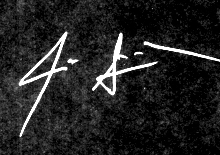
\includegraphics[width=0.8\linewidth]{original_1_1_transformed.png}
    \end{center}
    \caption{Genuine Signature}
    \label{fig:genuine}
\end{figure}
\begin{figure}[h]
    \begin{center}
        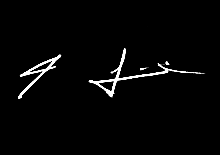
\includegraphics[width=0.8\linewidth]{forgeries_1_1_transformed.png}
    \end{center}
    \caption{Forged Signature}
    \label{fig:forge}
\end{figure}
\begin{figure}[h]
    \begin{center}
        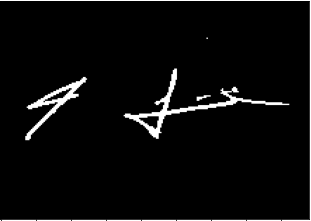
\includegraphics[width=0.8\linewidth]{improved_forge.png}
    \end{center}
    \caption{Forged Signature after FGSM Perturbation}
    \label{fig:improved_forge}
\end{figure}

% It appeared that the forge was just adding noise, as the genuine is noisy...
% So, I did this:
% $improved_forge[improved_forge < 1.0e-06] = 0.0$
% ...and got this:
% 0.06897393614053726
% which is just marginally more than the distance for genuine improved\_forge
% (so this background noise wasn't really helping that much)
% (maybe I should count how many elements were zeroed...)

% \subsubsection{Latent Vector Size}
% From Goodfellow's work, I think it might make sense to try playing with latent vector size...?
% Trained on 64, 128, and 256.
% The model sizes are: \_, \_, and \_.
% Training was way faster for the smaller models of course, but surprisingly so.
% 1000 per hour vs. \_ vs. \_...

% Training loss suggests that none of the models overfit.

% smaller models more accurate after one epoch, but also have many fewer parameters, so this could just mean that they are very underfit (we only did one epoch because training is so slow).
% Training is very slow for SigNet256.
% (I should introduce the names "SigNet64,128,256" earlier.)


% All of the confusion matrices can be seen in section \ref{sec:results}.

% maybe talk about playing with noise too if I actually get around to doing that properly...


% \section{just notes lol}
% I want to compute my metric of thresholds and prove hopefully prove that results in better accuracy than just optimizing the threshold (by trying all distances) on the training data.
% I want to compute a confusion matrix for the 3 models and then recompute it after applying perturbations.

% Hey, does DeepFool do what I'm talking about?
%     I should give it another glance before implementing...

% With any luck, I'll have results that say which latent vector size is best for accuracy and robustness to FGSM-like attacks.


% One interesting problem I ran into was I once manually saved a model just a batch or 2 after it call scheduler.step() (think it what caused it) and it performed much worse than I expected because the optimizer had made large changes... (I realized this because the val\_loss jumped up...)

\subsection{Discovery About CEDAR Dataset}\label{sec:cedar_flaw}
The images in the CEDAR dataset appear quite reasonable to the naked eye until they are inverted (so that black becomes white and vice versa).
There is an obvious difference in the background of the image of the genuine signature \ref{fig:genuine} when compared to that of the forged signature \ref{fig:forge}.

This was noticed early on during the research for this paper, but was not scrutinized until after all of the experiments had been performed and the bulk of the paper had been written.

The validation set images were analyzed as they are presented to the model: normalized, resized, and inverted.
The images were binned and then the bins were averaged over all of the images.
The resulting histogram can be seen in figure \ref{fig:hist_pixel_values}.

\begin{figure}[h]
    \begin{center}
        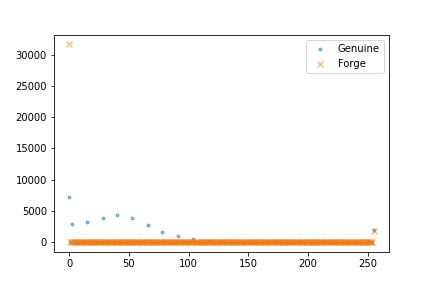
\includegraphics[width=0.8\linewidth]{mean_hist.png}
    \end{center}
    \caption{Histogram of Means of Binned Pixel Values}
    \label{fig:hist_pixel_values}
\end{figure}

This clearly shows that the images of genuine signatures have significantly different heuristics compared to the forged signatures.
In particular, the forged signatures have very few pixels with values in between 1 and 254, while the genuine signatures have many more.

With this realization, a very simple classifier was designed that examines an image and outputs whether or not there are more than 2000 pixels in it that have values in between 1 and 254.
This classifier was tested on the validation set and achieves 100\% accuracy.
While the threshold value (2000) was determined from the validation, the classifier also achieves 100\% accuracy when the threshold is set to 5000, so any value in that range will suffice.

Upon very closely inspecting the original images in the CEDAR dataset, it can be seen that the genuine and forged images are in fact different in this way.
Perhaps a different system was used for scanning the genuine and forged signatures.
